\documentclass{beamer}\usepackage[]{graphicx}\usepackage[]{color}
%% maxwidth is the original width if it is less than linewidth
%% otherwise use linewidth (to make sure the graphics do not exceed the margin)
\makeatletter
\def\maxwidth{ %
  \ifdim\Gin@nat@width>\linewidth
    \linewidth
  \else
    \Gin@nat@width
  \fi
}
\makeatother

\definecolor{fgcolor}{rgb}{0.345, 0.345, 0.345}
\newcommand{\hlnum}[1]{\textcolor[rgb]{0.686,0.059,0.569}{#1}}%
\newcommand{\hlstr}[1]{\textcolor[rgb]{0.192,0.494,0.8}{#1}}%
\newcommand{\hlcom}[1]{\textcolor[rgb]{0.678,0.584,0.686}{\textit{#1}}}%
\newcommand{\hlopt}[1]{\textcolor[rgb]{0,0,0}{#1}}%
\newcommand{\hlstd}[1]{\textcolor[rgb]{0.345,0.345,0.345}{#1}}%
\newcommand{\hlkwa}[1]{\textcolor[rgb]{0.161,0.373,0.58}{\textbf{#1}}}%
\newcommand{\hlkwb}[1]{\textcolor[rgb]{0.69,0.353,0.396}{#1}}%
\newcommand{\hlkwc}[1]{\textcolor[rgb]{0.333,0.667,0.333}{#1}}%
\newcommand{\hlkwd}[1]{\textcolor[rgb]{0.737,0.353,0.396}{\textbf{#1}}}%
\let\hlipl\hlkwb

\usepackage{framed}
\makeatletter
\newenvironment{kframe}{%
 \def\at@end@of@kframe{}%
 \ifinner\ifhmode%
  \def\at@end@of@kframe{\end{minipage}}%
  \begin{minipage}{\columnwidth}%
 \fi\fi%
 \def\FrameCommand##1{\hskip\@totalleftmargin \hskip-\fboxsep
 \colorbox{shadecolor}{##1}\hskip-\fboxsep
     % There is no \\@totalrightmargin, so:
     \hskip-\linewidth \hskip-\@totalleftmargin \hskip\columnwidth}%
 \MakeFramed {\advance\hsize-\width
   \@totalleftmargin\z@ \linewidth\hsize
   \@setminipage}}%
 {\par\unskip\endMakeFramed%
 \at@end@of@kframe}
\makeatother

\definecolor{shadecolor}{rgb}{.97, .97, .97}
\definecolor{messagecolor}{rgb}{0, 0, 0}
\definecolor{warningcolor}{rgb}{1, 0, 1}
\definecolor{errorcolor}{rgb}{1, 0, 0}
\newenvironment{knitrout}{}{} % an empty environment to be redefined in TeX

\usepackage{alltt}

% *****************************************************************************
% ADD HERE THE TOPIC OF THE LECTURE!
% \newcommand{\lecturetopic}{ALL LECTURE SLIDES}
\newcommand{\lecturetopic}{Day 8}
% *****************************************************************************



% turn off navigation symbols
\beamertemplatenavigationsymbolsempty

\title{\textbf{Data Analysis with R:} \\ \lecturetopic}
\author{Sonja Hartnack, Terence Odoch \& Muriel Buri}
\vspace{0.3cm}
\footnotesize
\institute{October 2017}
\date{ }

\setbeamertemplate{footline}[text line]{%
\parbox{\linewidth}{\vspace*{-1pt} \fontsize{3.5}{5}\selectfont Sonja Hartnack,
Terence Odoch \& Muriel Buri \hfill \lecturetopic \hfill \insertpagenumber}}

\usepackage{graphicx}
\usepackage{float}
\usepackage{animate}

\usepackage{verbatim}
\usepackage{url}
\usepackage{lmodern}
\usepackage{fancyhdr}
\usepackage{color}
\usepackage{amsmath, amssymb}
\usepackage{longtable}
\usepackage{lscape}
\usepackage{xspace}
\usepackage[normalem]{ulem}
% Use Palatino (URW Palladio) for most of the text\ldots
\usepackage[sc]{mathpazo}
% And Arial for the rest
\usepackage[scaled]{helvet}
\usepackage[latin1]{inputenc}
\usepackage{multicol} % A flexible tool to handle multicolumn documents
\usepackage{colortbl, xcolor} % enable colored rows in table
\usepackage{color} % enable colored rows in table
\usepackage{bibentry} % Include Full BibTeX Entry Inside Slides
\usepackage{nicefrac}
\usepackage{soul}

\setbeamertemplate{itemize items}[circle]

\usepackage{array}
\newcolumntype{L}[1]{>{\raggedright\let\newline\\\arraybackslash\hspace{0pt}}m{#1}}
\newcolumntype{C}[1]{>{\centering\let\newline\\\arraybackslash\hspace{0pt}}m{#1}}
\newcolumntype{R}[1]{>{\raggedleft\let\newline\\\arraybackslash\hspace{0pt}}m{#1}}

\graphicspath{{figures/}}
\usepackage[export]{adjustbox} % figure alignment
\usepackage{wrapfig} % allow for wrapfigure
\usepackage[margin=1cm]{caption}
\captionsetup{font=scriptsize, labelfont=scriptsize}

% change font family in footnote
\usepackage{footmisc}
\renewcommand*{\footnotelayout}{\tiny\sffamily}
% \renewcommand*{\footnotelayout}{\fontsize{3.5}{5}\selectfont\sffamily}

% change footer symbol
\usepackage{perpage}
\MakePerPage{footnote}
\renewcommand*{\thefootnote}{$\star$}

% change font sizes of frametitles
\setbeamerfont{frametitle}{size=\normalsize, series=\bfseries}
\setbeamerfont{framesubtitle}{size=\small, series=\bfseries}

% Settings for the references
\usepackage{natbib}
\usepackage{bibentry} % Include Full BibTeX Entry Inside Slides

% Writting the whole reference in ONE line.
% \def\newblock{\hskip .5em plus .33em minus .07em}

\setbeamerfont{title}{size=\LARGE}

\makeatletter
\def\mathcolor#1#{\@mathcolor{#1}}
\def\@mathcolor#1#2#3{%
\protect\leavevmode
\begingroup\color#1{#2}#3\endgroup
}
\makeatother

% *****************************************************************************

% {\usebackgroundtemplate{
\includegraphics[width=\paperwidth]{Printscreen_RLogo.png}}
{\usebackgroundtemplate{}}
\IfFileExists{upquote.sty}{\usepackage{upquote}}{}
\begin{document}

\bibliographystyle{plainnat}

% *****************************************************************************
% TITLE PAGE:
% *****************************************************************************

\begin{frame}[noframenumbering,plain]
\begin{columns}
\begin{column}{.3\linewidth}
\begin{center}
\includegraphics[height=.35\linewidth, width = 1.1\linewidth]{uzh_logo.pdf}
\end{center}
\end{column}
\begin{column}{0.2\linewidth}
\end{column}
\begin{column}{.3\linewidth}
\begin{center}
\includegraphics[height=.45\linewidth, width = .65\linewidth]{makere_logo.jpg}
\end{center}
\end{column}
\end{columns}
\titlepage
\end{frame}

\section{Day 8}
% \usebackgroundtemplate{
\includegraphics[width=\paperwidth]{Printscreen_RLogo.png}}
\usebackgroundtemplate{}
\begin{frame}
\frametitle{Acknowledgement}
\LARGE
We would like to thank \textbf{Beate Sick} for the inspiration given for these slides on \textit{missing values} and \textit{multiple imputation}.
\end{frame}

% \usebackgroundtemplate{
\includegraphics[width=\paperwidth]{Printscreen_RLogo.png}}
\usebackgroundtemplate{}
\begin{frame}
\frametitle{Missing Data\footnote{Thanks to \textbf{Beate Sick} for the
inspiration given for these slides on \textit{missing values} and
\textit{multiple imputation}.}}
\small
\begin{itemize}
\item \textbf{Nonresponse} occurs when information on all variables is missing
for a subset of the sample. Such non-responders may cause \textbf{selection bias},
as they effectively modify the study population to include only respondents.
\item \textbf{Item nonresponse} occurs when only some variables have missing
responses for a given individual.
\begin{itemize}
\item If missing probabilities of a predictor do not depend on the outcome,
then X is missing \textbf{nondifferentially}. Association between outcome
and missingness of a predictor can be tested!
\item \textbf{Differential missingness probabilities} depend on disease outcome.
This mainly arise in retrospective (e. g. case-control) studies.
If predictors (exposure) are measured prospectively before outcome
such dependency cannot occur in a direct way.
\end{itemize}
\end{itemize}
\end{frame}

\usebackgroundtemplate{
\includegraphics[width=\paperwidth]{Printscreen_RLogo.png}}
% \usebackgroundtemplate{}
\begin{frame}
\frametitle{Example: A study of HIV-positive people in NYC}
The \texttt{CHAIN} project was a longitudinal cohort study of people living with
HIV in New York City, which was recruited in 1994. Here we study a data subset
collected from $532$ subjects in the sixth round of interviews.
\begin{itemize}
\item \texttt{log\_virus}: Log of self reported viral load level (=0 if below detection limit).
\item \texttt{age}: The respondent's age at time of interview.
\item \texttt{income}: The respondent's family annual income.
\item \texttt{healthy}: A continuous scale of physical health (0-100).
\item \texttt{mental}: Measure of poor mental health: 0/1 = No/Yes.
\item \texttt{damage}: Ordered interval ($0$ to $5$) for CD4 count.
\item \texttt{treatment}: A three-level-ordered variable (0 = not currently
taking HAART therapy, 1 = taking HAART nonadherent, 2 = taking HAART adherent)
\end{itemize}
\end{frame}

\begin{frame}[fragile]
\frametitle{Reading in the \texttt{CHAIN} data set in R}


\begin{knitrout}
\definecolor{shadecolor}{rgb}{0.969, 0.969, 0.969}\color{fgcolor}\begin{kframe}
\begin{alltt}
\hlkwd{install.packages}\hlstd{(}\hlstr{"mi"}\hlstd{)}
\hlkwd{library}\hlstd{(}\hlstr{"mi"}\hlstd{)}
\hlkwd{data}\hlstd{(}\hlstr{"CHAIN"}\hlstd{)}
\hlstd{chain} \hlkwb{<-} \hlstd{CHAIN} \hlcom{# rename the data frame}
\hlkwd{names}\hlstd{(chain)}
\hlkwd{str}\hlstd{(chain)}
\hlkwd{summary}\hlstd{(chain)}
\end{alltt}
\end{kframe}
\end{knitrout}
\end{frame}

\begin{frame}[fragile]
\frametitle{Descriptive Statistics of the \texttt{CHAIN} data set in R}
\begin{knitrout}\tiny
\definecolor{shadecolor}{rgb}{0.969, 0.969, 0.969}\color{fgcolor}\begin{kframe}
\begin{alltt}
\hlkwd{hist}\hlstd{(chain}\hlopt{$}\hlstd{log_virus,} \hlkwc{ylim} \hlstd{=} \hlkwd{c}\hlstd{(}\hlnum{0}\hlstd{,} \hlnum{200}\hlstd{),} \hlkwc{col} \hlstd{=} \hlstr{"darkgray"}\hlstd{)}
\hlkwd{nrow}\hlstd{(chain)} \hlcom{# [1] 532}
\hlkwd{apply}\hlstd{(chain,} \hlnum{2}\hlstd{,} \hlkwa{function}\hlstd{(}\hlkwc{x}\hlstd{) \{}\hlkwd{sum}\hlstd{(}\hlkwd{is.na}\hlstd{(x))\})}
\hlcom{# log_virus       age    income   healthy    mental    damage treatment }
\hlcom{#       179        24        38        24        24        63        24}
\hlkwd{summary}\hlstd{(chain)}
\end{alltt}
\end{kframe}
\end{knitrout}
\end{frame}

% \usebackgroundtemplate{
\includegraphics[width=\paperwidth]{Printscreen_RLogo.png}}
\usebackgroundtemplate{}
\begin{frame}
\frametitle{Reasons for Item Nonresponse}
\begin{itemize}
\item Individuals may not respond to specific questions on sensitive issues
(e. g. questions on household income, drug abuse, ...).
\item Medical or occupational records may be incomplete.
Material might be spilled or reports might be lost in the mail.
\item Certain variables may be very expensive to measure for all study
participants.
\end{itemize}
\end{frame}

% \usebackgroundtemplate{
\includegraphics[width=\paperwidth]{Printscreen_RLogo.png}}
\usebackgroundtemplate{}
\begin{frame}
\frametitle{Missingness Mechanisms}
\begin{itemize}
\item \textbf{MCAR}: The missing completely at random (MCAR) mechanism assumes, that the
probability that a specific variable X is missing is does not depend on any
other factors.
\item \textbf{MAR}: The missing at random (MAR) mechanism assumes, that the probability that
a specific variable X is missing does not depend on the missing value of X,
but only on fully observed variables.
\item \textbf{MNAR}: Otherwise data are not missing at random (MNAR).
\end{itemize}
\begin{center}
\includegraphics[width=0.7\paperwidth]{missing_data.png}
\end{center}
\end{frame}

\usebackgroundtemplate{
\includegraphics[width=\paperwidth]{Printscreen_RLogo.png}}
% \usebackgroundtemplate{}
\begin{frame}[fragile]
\frametitle{Fitting a linear regression model to the \texttt{chain} data set}
\begin{knitrout}\tiny
\definecolor{shadecolor}{rgb}{0.969, 0.969, 0.969}\color{fgcolor}\begin{kframe}
\begin{alltt}
\hlcom{# R performs a complete case analysis using only rows with no NAs}
\hlstd{lm.mod.NA} \hlkwb{<-} \hlkwd{lm}\hlstd{(log_virus} \hlopt{~} \hlstd{age} \hlopt{+} \hlstd{income} \hlopt{+} \hlstd{healthy} \hlopt{+} \hlstd{mental} \hlopt{+}
                   \hlstd{damage} \hlopt{+} \hlstd{treatment,} \hlkwc{data} \hlstd{= chain)}
\hlkwd{summary}\hlstd{(lm.mod.NA)}
\end{alltt}
\begin{verbatim}
## 
## Call:
## lm(formula = log_virus ~ age + income + healthy + mental + damage + 
##     treatment, data = chain)
## 
## Residuals:
##     Min      1Q  Median      3Q     Max 
## -9.6015 -3.2863 -0.7366  3.5620 10.1283 
## 
## Coefficients:
##             Estimate Std. Error t value Pr(>|t|)    
## (Intercept) 17.37464    1.84104   9.437  < 2e-16 ***
## age         -0.10715    0.02914  -3.677 0.000276 ***
## income      -0.36671    0.11319  -3.240 0.001320 ** 
## healthy     -0.03627    0.01980  -1.832 0.067858 .  
## mentalyes    0.97222    0.53518   1.817 0.070191 .  
## damage      -1.18613    0.17947  -6.609 1.57e-10 ***
## treatment1  -2.05802    0.59768  -3.443 0.000649 ***
## treatment2  -2.21456    0.53367  -4.150 4.25e-05 ***
## ---
## Signif. codes:  0 '***' 0.001 '**' 0.01 '*' 0.05 '.' 0.1 ' ' 1
## 
## Residual standard error: 4.208 on 327 degrees of freedom
##   (197 observations deleted due to missingness)
## Multiple R-squared:  0.2506,	Adjusted R-squared:  0.2345 
## F-statistic: 15.62 on 7 and 327 DF,  p-value: < 2.2e-16
\end{verbatim}
\end{kframe}
\end{knitrout}
\end{frame}

\usebackgroundtemplate{
\includegraphics[width=\paperwidth]{Printscreen_RLogo.png}}
% \usebackgroundtemplate{}
\begin{frame}[fragile]
\frametitle{Checking the model assumptions for the \texttt{chain} data set}
\begin{knitrout}\tiny
\definecolor{shadecolor}{rgb}{0.969, 0.969, 0.969}\color{fgcolor}\begin{kframe}
\begin{alltt}
\hlcom{# R performs a complete case analysis using only rows with no NAs}
\hlkwd{par}\hlstd{(}\hlkwc{mfrow}\hlstd{=}\hlkwd{c}\hlstd{(}\hlnum{2}\hlstd{,}\hlnum{2}\hlstd{))}
\hlkwd{plot}\hlstd{(lm.mod.NA)}
\end{alltt}
\end{kframe}

{\centering 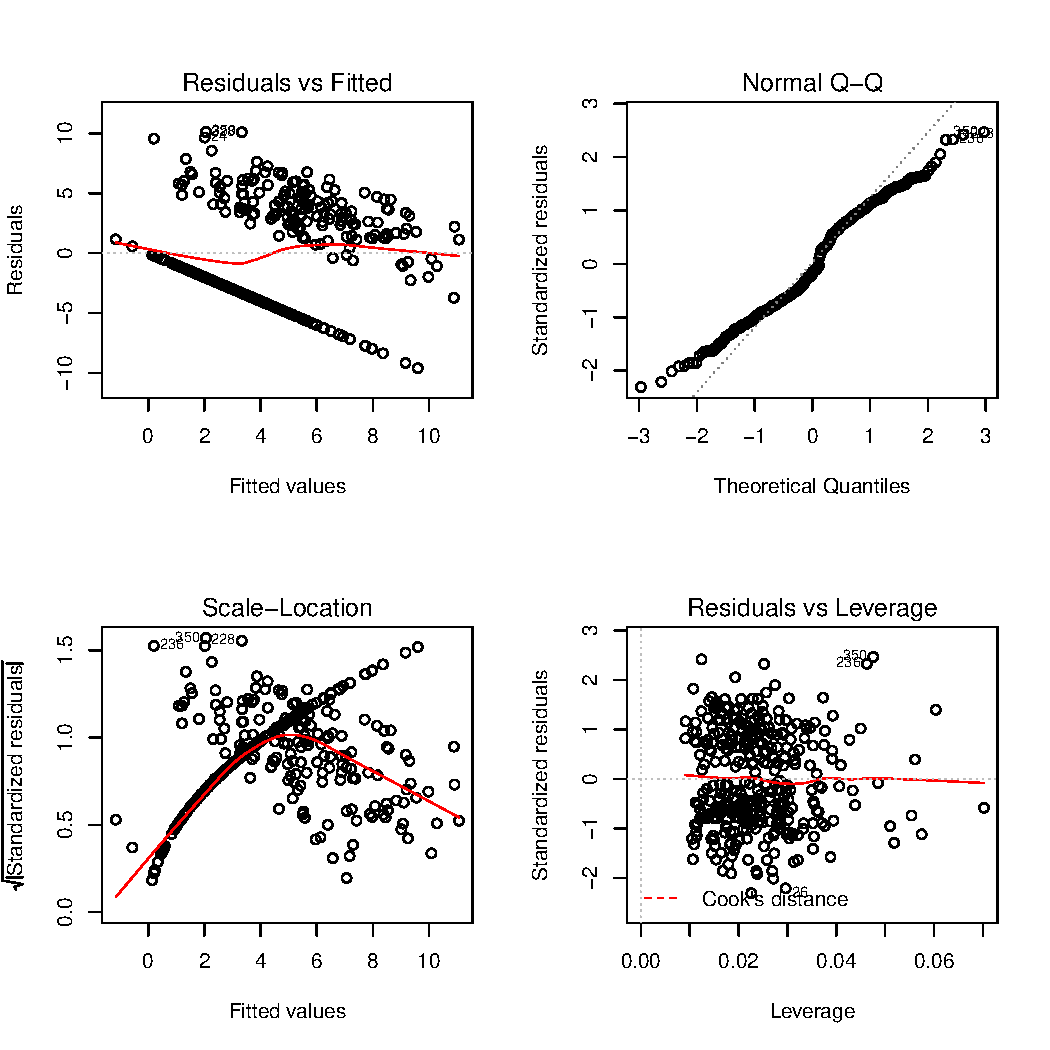
\includegraphics[width=0.7\linewidth]{figure/unnamed-chunk-6-1} 

}



\end{knitrout}
\end{frame}

\usebackgroundtemplate{
\includegraphics[width=\paperwidth]{Printscreen_RLogo.png}}
% \usebackgroundtemplate{}
\begin{frame}
\frametitle{Complete Data Analysis in linear regression}
\begin{itemize}
\item Complete case analysis uses only those records with complete observations
\item If the predictor values are missing nondifferentially, i. e. the probability
that a risk factor is missing does not depend on outcome y (disease status),
then complete case analysis produces valid regression coefficient estimates
\item If the predictor values are missing differentially the complete case
analysis can result substantial biased estimates.
\item There may also be a huge loss in precision (large CIs and $p$-values) if
a substantial part of the observations are omitted due to missing values.
\end{itemize}
\end{frame}

% \usebackgroundtemplate{
\includegraphics[width=\paperwidth]{Printscreen_RLogo.png}}
\usebackgroundtemplate{}
\begin{frame}
\frametitle{How are missing data treated?}
Simple solutions that often cause bias or other problems:
\begin{itemize}
\item Complete data analysis = Listwise deletion
\item Pairwise deletion
\item Single imputation (not discussed)
\item Last observation carried forward and baseline observation carried
forward (not discussed)
\end{itemize}
Better (but also more complex) approaches are
\begin{itemize}
\item \textbf{Multiple imputation}: mainly used to handle item missings - only
parts of the variables are missing
\item Inverse probability weighting (not discussed)
\end{itemize}
\end{frame}

% \usebackgroundtemplate{
\includegraphics[width=\paperwidth]{Printscreen_RLogo.png}}
\usebackgroundtemplate{}
\begin{frame}
\frametitle{Iterative methods to get an imputed data set}
\small
If we have missings in more than one variable:
\begin{itemize}
\item \textbf{Multivariate Imputation by Chained Equations (MICE, Van Buuren
and Oudshoorn (1999))} \newline
MICE imputes each variable stochastically using a regression model
conditional on all the others, iteratively cycling through all the variables that
contain missing data until convergence (''Gibbs sampling'').
In R we can use the mice package. The mice function assumes in default
settings linearity of associations among X variables and between X and Y in
the default setting, but specific forms of imputation models can be specified by
the user.
\item \textbf{An iterative nonparametric missing value imputation for mixed-type data}
can also be done by a method called missForest which is based on a random
forest approach. It can can cope with high-dimensional data and may
outperform MICE if complex interactions and nonlinear relations are
suspected. In R we can use the missForest package.
\end{itemize}
\end{frame}

\usebackgroundtemplate{
\includegraphics[width=\paperwidth]{Printscreen_RLogo.png}}
% \usebackgroundtemplate{}
\begin{frame}[fragile]
\frametitle{Iterative imputation based on \texttt{RandomForest}}
In the R package missForest (2012) is an iterative imputation method.
All imputation models are random forest models.
\begin{knitrout}\scriptsize
\definecolor{shadecolor}{rgb}{0.969, 0.969, 0.969}\color{fgcolor}\begin{kframe}
\begin{alltt}
\hlcom{# install.packages("missForest")}
\hlkwd{library}\hlstd{(}\hlstr{"missForest"}\hlstd{)}
\hlcom{# Nonparametric Missing Value Imputation using Random Forest}
\hlstd{chain.imp} \hlkwb{<-} \hlkwd{missForest}\hlstd{(chain,} \hlkwc{verbose} \hlstd{=} \hlnum{TRUE}\hlstd{,} \hlkwc{variablewise} \hlstd{=} \hlnum{TRUE}\hlstd{)}
\hlstd{chain.imp}\hlopt{$}\hlstd{OOBerror} \hlcom{# estimated imputation error for each variable}
\hlstd{chain.final.rf} \hlkwb{<-} \hlstd{chain.imp}\hlopt{$}\hlstd{ximp}
\hlkwd{dim}\hlstd{(chain.final.rf)} \hlcom{# [1] 532   7}
\hlkwd{apply}\hlstd{(chain.final.rf,} \hlnum{2}\hlstd{,} \hlkwa{function}\hlstd{(}\hlkwc{x}\hlstd{)\{}\hlkwd{sum}\hlstd{(}\hlkwd{is.na}\hlstd{(x))\})}
\hlcom{# log_virus       age    income   healthy    mental    damage treatment }
\hlcom{#         0         0         0         0         0         0         0 }
\hlstd{lm.mod.rf} \hlkwb{<-} \hlkwd{lm}\hlstd{(log_virus} \hlopt{~} \hlstd{age} \hlopt{+} \hlstd{income} \hlopt{+} \hlstd{healthy} \hlopt{+}
                   \hlstd{mental} \hlopt{+} \hlstd{damage} \hlopt{+} \hlstd{treatment,}
                \hlkwc{data} \hlstd{= chain.final.rf)}
\end{alltt}
\end{kframe}
\end{knitrout}
\begin{knitrout}\scriptsize
\definecolor{shadecolor}{rgb}{0.969, 0.969, 0.969}\color{fgcolor}\begin{kframe}
\begin{verbatim}
##   missForest iteration 1 in progress...done!
##     estimated error(s): 19.27203 69.01536 3.950885 145.4131 0.2755906 1.706025 0.523622 
##     difference(s): 0.000589767 0.009398496 
##     time: 1.022 seconds
## 
##   missForest iteration 2 in progress...done!
##     estimated error(s): 19.95495 66.14035 3.733105 145.3148 0.269685 1.701974 0.503937 
##     difference(s): 0.0003988586 0.01315789 
##     time: 0.761 seconds
## 
##   missForest iteration 3 in progress...done!
##     estimated error(s): 19.53889 64.51265 3.775952 141.5652 0.3051181 1.619511 0.4822835 
##     difference(s): 0.0002652466 0.01785714 
##     time: 0.891 seconds
## 
##   missForest iteration 4 in progress...done!
##     estimated error(s): 19.04295 67.92 3.762166 142.0383 0.2992126 1.668436 0.4822835 
##     difference(s): 0.000237364 0.009398496 
##     time: 0.801 seconds
## 
##   missForest iteration 5 in progress...done!
##     estimated error(s): 19.27342 65.25521 3.770057 138.6712 0.2874016 1.689657 0.4940945 
##     difference(s): 0.0003220432 0.01503759 
##     time: 1.037 seconds
\end{verbatim}
\end{kframe}
\end{knitrout}
\end{frame}

\usebackgroundtemplate{
\includegraphics[width=\paperwidth]{Printscreen_RLogo.png}}
% \usebackgroundtemplate{}
\begin{frame}
\frametitle{Main steps used in multiple imputation with \texttt{mice} in R}
\begin{figure}
\includegraphics[scale=0.6]{mice_steps.png}
\end{figure}
\end{frame}

\usebackgroundtemplate{
\includegraphics[width=\paperwidth]{Printscreen_RLogo.png}}
% \usebackgroundtemplate{}
\begin{frame}[fragile]
\frametitle{Multiple and iterative imputation with \texttt{mice} in R}
\begin{knitrout}\tiny
\definecolor{shadecolor}{rgb}{0.969, 0.969, 0.969}\color{fgcolor}\begin{kframe}
\begin{alltt}
\hlcom{# install.packages("mice")}
\hlkwd{library}\hlstd{(}\hlstr{"mice"}\hlstd{)}
\hlcom{# Multivariate Imputation by Chained Equations (MICE)}
\hlcom{# create 4 imputed data sets via mice}
\hlcom{# IMPUTE DATA}
\hlstd{chain.mice} \hlkwb{<-} \hlkwd{mice}\hlstd{(chain,} \hlkwc{m} \hlstd{=} \hlnum{4}\hlstd{,} \hlkwc{print} \hlstd{=} \hlnum{FALSE}\hlstd{,} \hlkwc{seed} \hlstd{=} \hlnum{2017}\hlstd{)}
\hlcom{# ANALYSE RESULTS WITH IMPUTED DATA}
\hlcom{# fit for each of the 4 data sets a linear regression}
\hlstd{fit.4.mice} \hlkwb{<-} \hlkwd{with}\hlstd{(chain.mice,} \hlkwd{lm}\hlstd{(log_virus} \hlopt{~} \hlstd{age} \hlopt{+} \hlstd{income} \hlopt{+} \hlstd{healthy} \hlopt{+}
                                     \hlstd{mental} \hlopt{+} \hlstd{damage} \hlopt{+} \hlstd{treatment))}
\hlcom{# check out the regression coefficients of the 4 fits}
\hlkwd{summary}\hlstd{(fit.4.mice)}
\hlcom{# POOL ANALYSIS RESULTS}
\hlcom{# pool the results of the 4 models with Rubin's rule}
\hlstd{lm.mod.mice} \hlkwb{<-} \hlkwd{pool}\hlstd{(fit.4.mice)}
\hlcom{# combined regression coefficients of the 4 fits}
\hlkwd{summary}\hlstd{(lm.mod.mice)}
\end{alltt}
\end{kframe}
\end{knitrout}

\end{frame}

\usebackgroundtemplate{
\includegraphics[width=\paperwidth]{Printscreen_RLogo.png}}
% \usebackgroundtemplate{}
\begin{frame}[fragile]
\frametitle{Comparison of results: Complete case vs. \texttt{missForest}}
\begin{knitrout}\tiny
\definecolor{shadecolor}{rgb}{0.969, 0.969, 0.969}\color{fgcolor}\begin{kframe}
\begin{alltt}
\hlkwd{round}\hlstd{(}\hlkwd{summary}\hlstd{(lm.mod.NA)}\hlopt{$}\hlstd{coef,} \hlnum{2}\hlstd{)}
\end{alltt}
\begin{verbatim}
##             Estimate Std. Error t value Pr(>|t|)
## (Intercept)    17.37       1.84    9.44     0.00
## age            -0.11       0.03   -3.68     0.00
## income         -0.37       0.11   -3.24     0.00
## healthy        -0.04       0.02   -1.83     0.07
## mentalyes       0.97       0.54    1.82     0.07
## damage         -1.19       0.18   -6.61     0.00
## treatment1     -2.06       0.60   -3.44     0.00
## treatment2     -2.21       0.53   -4.15     0.00
\end{verbatim}
\begin{alltt}
\hlkwd{round}\hlstd{(}\hlkwd{summary}\hlstd{(lm.mod.rf)}\hlopt{$}\hlstd{coef,} \hlnum{2}\hlstd{)}
\end{alltt}
\begin{verbatim}
##             Estimate Std. Error t value Pr(>|t|)
## (Intercept)    15.19       1.22   12.46     0.00
## age            -0.09       0.02   -4.31     0.00
## income         -0.34       0.08   -4.15     0.00
## healthy        -0.03       0.01   -2.15     0.03
## mentalyes       1.03       0.36    2.89     0.00
## damage         -1.08       0.12   -8.62     0.00
## treatment1     -1.63       0.40   -4.11     0.00
## treatment2     -1.70       0.36   -4.68     0.00
\end{verbatim}
\end{kframe}
\end{knitrout}
\end{frame}

\usebackgroundtemplate{
\includegraphics[width=\paperwidth]{Printscreen_RLogo.png}}
% \usebackgroundtemplate{}
\begin{frame}[fragile]
\frametitle{Comparison of results: Complete case vs. \texttt{mice}}
\begin{knitrout}\tiny
\definecolor{shadecolor}{rgb}{0.969, 0.969, 0.969}\color{fgcolor}\begin{kframe}
\begin{alltt}
\hlkwd{round}\hlstd{(}\hlkwd{summary}\hlstd{(lm.mod.NA)}\hlopt{$}\hlstd{coef,} \hlnum{2}\hlstd{)}
\end{alltt}
\begin{verbatim}
##             Estimate Std. Error t value Pr(>|t|)
## (Intercept)    17.37       1.84    9.44     0.00
## age            -0.11       0.03   -3.68     0.00
## income         -0.37       0.11   -3.24     0.00
## healthy        -0.04       0.02   -1.83     0.07
## mentalyes       0.97       0.54    1.82     0.07
## damage         -1.19       0.18   -6.61     0.00
## treatment1     -2.06       0.60   -3.44     0.00
## treatment2     -2.21       0.53   -4.15     0.00
\end{verbatim}
\begin{alltt}
\hlkwd{round}\hlstd{(}\hlkwd{summary}\hlstd{(lm.mod.mice)[,}\hlkwd{c}\hlstd{(}\hlnum{1}\hlstd{,}\hlnum{2}\hlstd{,}\hlnum{3}\hlstd{,}\hlnum{5}\hlstd{)],} \hlnum{2}\hlstd{)}
\end{alltt}
\begin{verbatim}
##               est   se     t Pr(>|t|)
## (Intercept) 15.60 1.57  9.95     0.00
## age         -0.09 0.03 -3.25     0.00
## income      -0.35 0.11 -3.09     0.00
## healthy     -0.03 0.02 -1.55     0.13
## mental2      1.16 0.56  2.06     0.05
## damage      -1.01 0.17 -5.76     0.00
## treatment2  -2.27 0.56 -4.06     0.00
## treatment3  -2.13 0.52 -4.10     0.00
\end{verbatim}
\end{kframe}
\end{knitrout}
\end{frame}

% \usebackgroundtemplate{
\includegraphics[width=\paperwidth]{Printscreen_RLogo.png}}
\usebackgroundtemplate{}
\begin{frame}
\frametitle{Multiple Imputation - the principle idea}
\begin{itemize}
\item $m$ imputed data sets are created instead of a single imputed data set
(Rubin has shown that often $m = 5$ to $10$ is sufficient)
\item To create the m imputed data sets take random draws from the predictive
distribution from an imputation model, e.g. 5 times or do iterative imputation
several times with different starting values and draw random draws.
\item The variation among the m imputations reflects the uncertainty with which the
missing values can be predicted from the observed data.
\item With each completed data set the planned analysis is performed.
\item The results from the different analyses are then combined using Rubin's rule properly taking into account the uncertainty in the imputed values.
\end{itemize}
\end{frame}

% \usebackgroundtemplate{
\includegraphics[width=\paperwidth]{Printscreen_RLogo.png}}
\usebackgroundtemplate{}
\begin{frame}
\frametitle{Summary on imputation}
Missing data lead to
\begin{itemize}
\item Inefficient analyses of research questions
\item Difficulties in interpretation when analyses differ in numbers of subjects
\item Possible bias in regression coefficients
\end{itemize}
\begin{itemize}
\item \textbf{Imputation methods make the assumption of MAR}
\item The MAR assumption is not testable, but becomes more reasonable with
imputation models that include a wide range of variables.
\end{itemize}
\begin{itemize}
\item \textbf{Multiple imputation is recommended and superior to complete data analysis.}
\item Single imputation methods are also reasonable for prediction.
\end{itemize}
\end{frame}

% \usebackgroundtemplate{
\includegraphics[width=\paperwidth]{Printscreen_RLogo.png}}
\usebackgroundtemplate{}
\begin{frame}
\frametitle{Summary for Anna Mary}
\begin{itemize}
\setlength\itemsep{1.5em}
\item ONE continuous vs. ONE categorical variable (2 levels)
\begin{itemize}
\item \texttt{t.test(...)}
\end{itemize}
\item ONE continuous vs. ONE categorical variable ($\geq$ 2 levels)
\begin{itemize}
\item \texttt{aov(...)}
\end{itemize}
\item ONE categorical variable (2 levels) vs. ONE categorical variable (2 levels) $\rightarrow$ 2 x 2 table
\begin{itemize}
\item \texttt{chisq.test(...)}
\item \texttt{fisher.test(...)}
\end{itemize}
\end{itemize}
\vspace{0.3em}
\LARGE $\rightarrow$ Regression:  \texttt{lm(...)} \& \texttt{glm(...)}
\end{frame}

% CONTRASTS
% https://www.r-bloggers.com/using-and-interpreting-different-contrasts-in-linear-models-in-r/
% https://rcompanion.org/rcompanion/h_01.html
% http://www.stat.wisc.edu/courses/st850-lindstro/handouts/contrasts.pdf

% *****************************************************************************

\end{document}

% as.numeric.factor <- function(x) {as.numeric(levels(x))[x]}
